\chapter{研究现状} \label{chap:related}
%本文根据在视觉目标跟踪中使用方法的不同,将视觉目标跟踪方法分为传统的基于相关滤波的视觉目标跟踪方法和基于深度学习的视觉目标跟踪方法。
%其中,基于相关滤波的视觉目标跟踪方法本质上采用岭回归学习,由于其使用循环移位的特殊采样方式,可以通过快速离散傅里叶变换在频域中高效求解,具有较快的运行速度,成为了深度学习时代之前最具代表性的视觉目标跟踪算法。
近年来,
%深度学习方法在视觉目标跟踪任务中的应用越来越广泛。
基于深度学习的视觉目标跟踪方法,尤其是基于卷积神经网络的视觉目标跟踪方法,受到学术和工业界的广泛关注。
%接下来,本章将分别对传统的基于相关滤波的视觉目标跟踪方法和基于深度学习的视觉目标跟踪方法进行系统的介绍。
本章主要介绍基于深度学习的目标跟踪方法的研究现状,将基于深度学习的跟踪器划分为以下几种类别:基于深度特征的相关滤波跟踪器、基于生成对抗网络的跟踪器、基于图卷积网络的跟踪器、基于循环神经网络的跟踪器、基于脉冲神经网络的跟踪器、基于孪生网络的跟踪器、基于强化学习的跟踪器、基于元学习的跟踪器、基于无监督学习的跟踪器、基于注意力机制的跟踪器和基于串并联或级联结构的跟踪器。

\section{基于深度特征的相关滤波跟踪器}
相关滤波跟踪器是传统跟踪器中的代表之一。基于相关滤波的视觉目标跟踪方法本质上采用岭回归学习,由于其使用循环移位的特殊采样方式,可以通过快速离散傅里叶变换在频域中高效求解,具有较快的运行速度,成为了深度学习时代之前最具代表性的视觉目标跟踪算法。
%相关滤波跟踪的基本思想是,设计一个滤波模板,利用该模板与目标候选区域做相关运算,最大输出响应的位置即为当前帧的目标位置。该跟踪器通过利用离散傅里叶变换以有效的方式利用了跟踪样本的所有空间偏移。
%基于相关滤波的视觉目标跟踪算法将空域内的密集搜索通过相关滤波的方式转化为频域内的点积运算,得益于快速傅里叶变换,在频域内高效进行表观建模,跟踪实时性好,能够达到很高的帧率。
Bolme 等人 \cite{MOSSE} 首次将相关滤波与自适应目标跟踪相结合,提出 MOSSE 跟踪算法,该跟踪器以每秒 669 帧的速度运行,可以抵抗光照、尺度、姿势的变化和目标的非刚性形变。
CSK 跟踪器 \cite{Henriques2012ExploitingTC} 通过采用图像子窗口的循环结构并使用快速傅里叶变换(fast Fourier transform,FFT)快速合并来自所有子窗口的信息,对 MOSSE 跟踪器进行了改进。此外,文献 \cite{Henriques2012ExploitingTC} 表明,使用核技巧可以像在原始图像空间中一样高效地完成非线性空间中的分类。
在文献 \cite{Danelljan2014AdaptiveCA} 中,Danelljan 等人通过学习有关多维颜色属性的多通道滤波器来改进 CSK 跟踪器。为了避免由于颜色属性的高维而导致的计算开销,Danelljan 等人 \cite{Danelljan2014AdaptiveCA} 提出了一种自适应维降技术,可以将原始的 11 维特征减少到只有 2 维。
后来,Henriques 等人 \cite{henriques2014high-speed} 为大量图像补丁提出了一种分析模型,使用离散傅里叶变换将模型对角线化,此操作可以将存储和计算量减少几个数量级。

传统的相关滤波跟踪器通常采用手工设计的特征或底层特征,这限制了相关滤波器的潜力。随着深度学习时代的到来,有很多相关滤波跟踪器尝试使用深度特征代替底层特征,并取得了性能的提升。在文献 \cite{CF2} 中,Ma 等人利用从深度卷积神经网络中提取的特征进行相关滤波的学习,来提高跟踪精度和鲁棒性。作者利用最后一个卷积层的输出对目标的语义信息进行编码,使得跟踪器对于目标的表观变化具有鲁棒性。但是,由于空间分辨率太粗糙,无法精确定位目标。相反,较浅的卷积层提供了更精确的定位信息。因此作者在每个卷积层上自适应学习相关滤波器,以对目标表观进行编码。在文献 \cite{danelljan2016beyond} 中,Danelljan 等人在常规相关滤波跟踪器框架的基础上,提出了一种用于训练连续卷积滤波器的算法。作者采用隐式插值模型来解决连续空间域中的学习问题。该模型可实现对于多种分辨率的特征图的有效集成。此外,该方法能够进行亚像素定位,有利于提高跟踪的精确性。
\section{基于生成对抗网络的跟踪器}
生成对抗网络(generative adversarial network,GAN)可以利用卷积神经网络从随机噪声生成逼真的图像。生成对抗网络包含两个子网,一个充当生成器,另一个充当判别器。 生成器旨在合成图像以欺骗判别器,而判别器则试图正确区分真实图像和生成器合成的图像。通过相互竞争来同时训练生成器和判别器。对抗学习的优势在于,所训练的生成器可以生成与训练样本相似的图像统计信息,从而使判别器无法区分。生成对抗网络的进步吸引了包括目标跟踪在内的各种计算机视觉应用的关注。在文献 \cite{VITAL} 中,Song 等人利用生成对抗网络产生的样本辅助跟踪器的学习。文章指出,由于以下问题,现有视觉跟踪器的性能可能会受到限制:(1)采用密集采样策略生成的正样本会降低样本的多样性,(2)即使收集到大规模的训练数据集,具有挑战性的训练数据也是有限的。作者提出了 VITAL 算法来通过对抗学习解决这两个问题。为了增加正样本,作者使用一个生成网络随机生成模板,这些模板用于自适应过滤输入特征以捕获各种表观变化。通过对抗学习获得的模板,可以提供鲁棒的目标特征。此外,为了解决类别不平衡的问题,作者提出了一个高阶成本敏感损失,从而有助于训练分类网络。在文献 \cite{SINT++} 中,Wang 等人通过对抗生成学习产生难例正样本进行跟踪。具体来说,作者假设目标都位于流形上,因此,引入正样本生成网络,通过遍历已构建的目标流形来采样大量训练数据。生成的各种目标图像可以丰富训练数据集并增强目标跟踪器的鲁棒性。为了使跟踪器对遮挡更加鲁棒,作者提出了一个变换网络,该网络可以生成用于跟踪算法的难例样本。%SINT++: robust visual tracking via adversarial positive instance generation
受生成对抗网络 \cite{GAN} 和条件生成对抗网络 \cite{cGAN} 启发,Zhao 等人 \cite{AdversarialDeep} 提出了一种跟踪器,通过对抗学习共同优化了回归 CNN(R-Net)和分类 CNN(C-Net)。在训练阶段,分别为 R-Net 和 C-Net 创建二元组和三元组训练集。二元组训练集包含模板图像和搜索图像。通过二元组训练集,可以训练 R-Net 生成一个响应图,该响应图反映目标在搜索图像中的位置和大小。三元组训练集包含模板图像、搜索图像和响应图。利用三元组训练集对 C-Net 进行训练,以区分响应图是否能够反映搜索图像中目标的位置和大小。在测试阶段,首先根据上一帧中的目标位置,在当前帧提取数个搜索图像作为候选。二元组集包含一个搜索图像和一个模板图像。R-Net 基于这些二元组集生成一组响应图。然后,C-Net 根据三元组来选择最佳响应图。最后,使用最佳响应图在当前帧中定位目标。% Adversarial Deep Tracking

\section{基于图卷积网络的跟踪器}
图卷积神经网络(graph convolutional network,GCN)是一种能对图数据进行深度学习的方法。在目标跟踪中,图卷积网络用于捕获目标样本的结构特征。在文献 \cite{gao2019graph} 中,Gao 等人指出时空信息可以用于增强目标的特征表示,同时上下文信息对于目标的定位很重要。为了全面利用历史目标样本的时空结构并从上下文信息中受益,作者提出了一种用于高性能视觉跟踪的新型图卷积跟踪(GCT)方法。具体而言,GCT 将两种类型的图卷积网络整合到用于目标表观建模的孪生框架中。作者采用时空 GCN 来建模历史目标样本的结构化表示。而上下文 GCN 被设计为利用当前帧的上下文来学习用于目标定位的自适应特征。在文献 \cite{tu2019visual} 中,Tu 等人同样使用 GCN 模块来学习目标跟踪的结构特征。首先,作者利用双流网络提取异构特征。然后,作者采用 GCN 模块来构建结构化的信息要素。

\section{基于循环神经网络的跟踪器}
循环神经网络(recurrent neural network,RNN)是一类以序列(sequence)数据为输入,在序列的演进方向进行递归(recursion)且所有节点(循环单元)按链式连接的神经网络。RNN 在建模序列数据方面引起了越来越多的关注,例如多语言机器翻译、动作识别、场景解析、语音识别等。最近,传统的 RNN 演进为更复杂的结构模型,例如二维 RNN \cite{shuai2015quaddirectional}、多维 RNN \cite{stollenga2015parallel}、树 RNN \cite{tai2015improved} 等。在目标跟踪中,可利用 RNN 建模目标的复杂远程依赖关系。
RTT \cite{RTT} 尝试识别并利用对整个跟踪过程有益的可靠部件。为了解决遮挡问题并识别可靠的部件,RTT 使用了多方向循环神经网络,从多个方向遍历候选空间区域,从而捕获远程上下文线索。从 RNN 生成的置信度图用于抑制背景噪声,同时充分利用来自可靠部分的部件,从而自适应地进行判别相关滤波器的学习。%Recurrently target-attending tracking
在文献 \cite{SpatiallySupervised} 中,Ning 等人利用循环神经网络学习目标的历史位置信息,利用卷积神经网络学习目标的视觉特征。受目标检测中边框回归方法的启发,作者研究了时域中的长短时记忆(long short-term memory,LSTM)的回归能力,并提出将卷积网络产生的高级视觉特征与位置信息相结合的方法。
%与将二进制分类用于区域候选的现有基于深度学习的跟踪器不同,作者使用回归来直接预测卷积层和循环单元处的跟踪位置。
与仅基于历史位置信息的卡尔曼滤波器或采用时间预测方法的现有跟踪方法相比,作者提出的循环卷积模型能够同时考虑历史位置信息及过去帧的鲁棒视觉特征。% spatially supervised recurrent convolutional neural networks for visual object tracking
在文献 \cite{gordon2018re} 中,Gordon 等人提出了一种能够将时间信息整合到模型中的实时目标跟踪器。该跟踪器不专注于一组有限目标或在测试时训练一个模型来跟踪特定目标,而是在大量不同的目标上预先训练一个通用跟踪器,并进行实时的在线更新。%Re al-Time Recurrent Regression Networks for Visual Tracking of Generic Objects
在文献 \cite{RecurrentFilter} 中,Yang 等人
%通过保持目标表观并通过长短期记忆(LSTM)网络跟踪过滤器,
提出了循环滤波器学习算法。作者采用全卷积神经网络编码目标表观信息,同时保留目标的空间结构。作者认为,将 CNN 特征图展平为向量后传递给 LSTM 会使目标的结构变得模糊。因此,作者将 LSTM 的输入、输出单元和隐藏状态更改为特征图,并在网络中使用卷积层而不是全连接层。卷积 LSTM 的输出是一个滤波器,将其与下一帧的特征图进行卷积以生成目标响应图。%Recurrent Filter Learning for Visual Tracking
在文献 \cite{PRNet} 中,Ma 等人认为图像中不同尺度的上下文提供了不同的空间关系线索,应以恰当方式进行充分利用进行视觉目标跟踪。为利用全面的上下文线索,作者提出了金字塔循环神经网络。在每种上下文尺度中,使用多达 8 个方向的 RNN 收集目标的上下文信息。每个定向 RNN 都可以提取目标各部分之间的上下文相关性,这使其对背景信息和相似物体更具判别性。 % Multi-Scale Recurrent Tracking via Pyramid Recurrent Network and Optical Flow
\section{基于脉冲神经网络的跟踪器}% SiamSNN: Spike-based Siamese Network for Energy-Efficient and Real-time Object Tracking
卷积神经网络在多种计算机视觉应用中均表现出良好的性能。然而,由于高计算成本和高能耗,难以在诸如移动设备之类的嵌入式系统上使用 深度卷积神经网络。为此,研究人员提出了许多体积较小的网络 \cite{wei2018quantization},并实现了较好的性能。然而,在资源受限的系统中仍然存在计算能力不足的问题。作为替代方案,脉冲神经网络(spiking neural network,SNN)基于脉冲——这是一种发生在时间点上的离散事件——而非常见的连续值来传输信息。SNN 中的脉冲神经元仅在其膜电位超过特定阈值时才触发脉冲,这会稀疏地激活网络中的神经元以节省能量。SNN 被视为第三代人工神经网络。
最新的跟踪模型 \cite{SiamFC,SiamRPN} 需要高性能图形处理单元(graphics processing unit,GPU),这会导致计算和功耗需求急剧增加,因此难以部署至嵌入式平台 \cite{basu2018low}。借助 SNN 的低功耗计算,实现基于脉冲神经网络的跟踪器对于在嵌入式系统上部署节能跟踪算法具有重要意义。在文献 \cite{SiamSNN} 中,Luo 等人提出了 SiamSNN 以利用深度 SNN 进行目标跟踪,具有延迟短且精度损失低等特点。这是将深度 SNN 应用于具有复杂场景的数据集上的目标跟踪的首次成功尝试。具体来说:首先,作者利用脉冲序列的时间信息,提出了一种混合相似度估计方法来构建基于脉冲的相关层,以脉冲方式有效评估两个特征图之间的相似度。其次,作者提出了一种新型编码方案来优化输出脉冲序列的时间分布,从而改善性能并缩短时延。
在文献 \cite{DashNet} 中,Yang 等人提出了一种用于 SNN 跟踪的训练方法。作者为基于事件驱动的数据集开发了 SNN 模型,并为跟踪提供了准确的信息表示。
%据我们所知,这是探索针对跟踪和检测任务的SNN直接训练的第一项工作。
%•用于高速跟踪的混合人工和峰值模型。
具体来说,作者提出了一种混合模式,通过注意力机制共同处理来自卷积神经网络的同步信号和来自脉冲神经网络的事件驱动信号,在神经芯片上以 2083 帧每秒的速度实现了较好的跟踪性能。%https://arxiv.org/pdf/1909.12942.pdf
\section{基于孪生网络的跟踪器}
孪生网络是一种用于度量学习的有监督模型。孪生网络具有两个参数共享的子网络,可以学习两幅输入图像之间的特征相似性。由于优越的性能,基于孪生网络的跟踪器已经成为当前目标跟踪领域的主流。在 SiamFC \cite{SiamFC} 中,Bertinetto 等人证明了使用孪生网络解决跟踪问题的有效性。具体来说,作者训练了一个孪生网络以在较大的搜索图像中定位模板图像。利用互相关操作以滑动窗口的方式获得目标位置的响应图,从而对目标进行实时定位。在 SiamRPN \cite{SiamRPN} 中,跟踪器由用于特征提取的孪生网络和包括分类分支和回归分支的区域生成网络(region proposal network,RPN)组成。受益于跟踪器的改进,传统的多尺度测试和在线微调可以被丢弃。SiamRPN++ \cite{SiamRPN++} 基于其在分类和状态估计分解中的成功经验,通过一种简单而有效的空间感知采样策略进一步突破了严格的平移不变性的限制,并成功地训练了 ResNet \cite{he2016deep} 驱动的孪生跟踪器,从而显着提高了性能。
%除了这些基于锚框的方法以外,SiamFC++ \cite{SiamFC++} 通过考虑无歧义评分,无目标目标规模/比率分布和估计质量评估准则,进一步设计了无锚跟踪器 。
\subsection{针对孪生网络跟踪器的对抗攻击}
大量研究表明,卷积神经网络容易受到对抗攻击 \cite{Deepsec}。在文献 \cite{intriguing} 中,Szegedy 等人首先展示了对抗性攻击的存在。Goodfellow 等人 \cite{FGSM} 提出了一种有效的单步对抗攻击方法 FGSM,后来通过迭代方法 \cite{kurakin2017adversarial} 和动量项 \cite{dong2018boosting} 对 FGSM 进行了改进。类似地,Papernot 等人 \cite{papernot2016limitations} 提出了基于雅可比的显着图攻击,具有较高攻击成功率,而 C&W 算法 \cite{carlini2017towards} 通过优化方法在不同范数下实现了有效攻击。近年来,对抗攻击进一步扩展到自然语言处理 \cite{generating} 和图像目标检测 \cite{wei2019transferable} 等任务中。
最近的研究表明,基于卷积神经网络的孪生跟踪器同样容易受到对抗攻击。在文献 \cite{SPARK} 中,Guo 等人正式提出了视觉目标跟踪的对抗性攻击问题,即,在线生成无法感知的扰动以误导跟踪器,使跟踪器预测不正确的轨迹或指定的轨迹。此外,作者提出了一种空间感知的在线增量攻击方法 SPARK,该方法可在线产生难以察觉的扰动以执行快速有效的攻击。SPARK \cite{SPARK} 通过使用过去帧中的信息计算增量扰动,从而对孪生跟踪器进行攻击。但是,SPARK 需要通过繁琐的迭代方案为每个搜索图像生成独特的对抗样本,这对于实时在线跟踪算法而言非常耗时。在文献 \cite{chen2020one} 中,Chen 等人提出了一种具有双重损失和双重注意力机制的新型攻击方法,在初始帧为模板图像产生对抗性扰动。作者提出的攻击方法的优化目标包括两个损失,每个损失都与精心设计的注意力权重相结合,以进一步提高攻击能力。
PAT \cite{PAT} 通过白盒攻击生成物理对抗纹理,以引导跟踪器在被跟踪目标移到该纹理前面时锁定跟踪框。然而,PAT 仅通过攻击跟踪器 GOTURN \cite{GOTURN} 来验证其方法的有效性,该跟踪器与主流的目标跟踪算法相比在性能上有较大差距。
RTAA \cite{RTAA} 利用时间信息为视频的每帧图像生成微小扰动。RTAA 仅可使跟踪器无法正确跟踪目标,却不能使跟踪器输出任意的复杂轨迹。
在文献 \cite{TTP} 中,Nakka 等人提出仅使用模板图像生成一个时间可传递的扰动,然后将其添加到每个搜索图像中,以进行实时攻击。然而,该方法针对每个视频都需要运行对抗生成网络以生成特定于视频的扰动。%仍然需要为每个视频生成扰动,并且需要运行对抗生成网络以产生扰动。
%其有针对性的攻击设置需要从网络推理的多次运行中获得不同的扰动。
当计算资源有限或无法访问时,便不适用于攻击现实世界的在线跟踪系统。
\section{基于强化学习的跟踪器}
强化学习(reinforcement learning,RL)的目标是学习一种通过最大化未来累积奖励来决定动作序列的策略。
在文献 \cite{yun2017action} 中,Yun 等人提出了一种新型跟踪器,该跟踪器顺序执行通过深度强化学习而学到的动作来跟踪目标。与使用深层网络的现有跟踪器相比,所提出的跟踪器旨在实现轻量级计算以及较好的跟踪精度。控制动作的深层网络使用各种训练序列进行了预训练,并在跟踪过程中进行了微调,以在线适应目标和背景变化。 %  Action-decision networks for visual tracking with deep reinforcement learning
在文献 \cite{supancic2017tracking} 中,Supancic 等人将跟踪形式化为部分可观察的决策过程来学习最佳决策策略。作者使用深度强化学习算法学习策略,这些算法仅在运动轨迹出现问题时才需要监督(奖励信号)。作者证明稀疏的奖励有利于快速地对海量数据集进行训练。 %  Tracking as online decision-making: Learning a policy from streaming videos with reinforcement learning
在文献 \cite{DeepReinforcement} 中,Zhang 等人认为跟踪问题可以看作是一个顺序决策过程,而历史语义编码了与将来决策密切相关的信息。因此,作者提出了一种循环神经网络与强化学习算法相结合的神经网络跟踪器,将跟踪模型表示为循环神经网络代理,并用强化学习算法对模型进行训练,以学习良好的跟踪策略,并从长远来看最大化跟踪性能。% Deep Reinforcement Learning for Visual Object Tracking in Videos
在文献 \cite{RealTimeVisual} 中,Choi 等人提出了一种新型实时视频跟踪算法,该算法基于深度强化学习来指定模板选择策略。跟踪算法利用此策略来选择适当的模板以跟踪给定的视频帧序列。模板选择策略通过对跟踪基准数据集中随机生成的大量训练样本使用简单的策略梯度方法进行学习。% Real-time visual tracking by deep reinforced decision making
在文献 \cite{HierarchicalTracking} 中,Zhong 等人利用从深度强化学习中学到的数据驱动的运动模型为跟踪器提供目标的粗略定位,通过将运动搜索表述为强化学习中的动作决定问题,跟踪器利用基于循环神经网络的深度 Q 网络来有效地学习数据驱动的搜索策略。在每一帧中,运动模型将以先前估计位置为中心的候选图像块迭代地作为输入,并生成每个动作的概率作为输出。在每次迭代中,选择一个最佳动作来移动目标边界框。% Hierarchical Tracking by Reinforcement Learning-Based Searching and Coarse-to-Fine Verifying
在文献 \cite{LearningPolicies} 中,Huang 等人将自适应跟踪问题形式化为决策过程,并学习一个代理来决定是否以较高的置信度在网络的浅层上定位目标,或者继续处理网络的后续层。具体来说,该代理学习在每一层上找到目标,并确定是否有足够的信心在此处输出和停止。如果没有,将前进到下一层继续进行判断,通过选择最佳的网络层进行跟踪。该代理以强化学习的方式进行离线训练,并可在单个 CPU 上以接近 23 帧每秒的跟踪速度进行目标跟踪。% Learning Policies for Adaptive Tracking with Deep Feature Cascades
\section{基于元学习的跟踪器} %https://openaccess.thecvf.com/content_CVPR_2020/papers/Wang_Tracking_by_Instance_Detection_A_Meta-Learning_Approach_CVPR_2020_paper.pdf
元学习的目标是针对各种学习任务训练模型,以便仅使用少量训练样本即可解决新的学习任务 \cite{MAML}。如果将目标跟踪视为实例检测任务,跟踪器将接受各种实例检测任务的训练,以便仅使用来自初始或先前帧的一个或几个训练样本即可快速学习如何检测新实例,因此元学习可以用于设计视觉目标跟踪算法。模型无关的元学习(model-agnostic meta-learning,MAML)\cite{MAML} 是元学习的重要算法,该算法可令网络学习一组适用于微调的良好初始化参数。在训练期间,MAML 显式训练模型的参数,当应用于新任务时,利用少量训练数据和几次梯度下降步骤即可在该任务上获得良好的泛化性能。 MAML 的重要优点是,它与通过梯度下降训练的任何模型兼容,并且适用于各种不同的学习问题。
% 因此,MAML 是将元学习应用于目标跟踪的理想算法,该想法是将任何高级对象检测器(经过梯度下降训练)转换为跟踪器。
最近,研究人员提出了多种方案以完善 MAML。MAML++ \cite{MAML++} 引入了一些技巧来稳定 MAML 的训练。MetaSGD \cite{MetaSGD} 针对每个参数训练可学习的学习率。
在目标跟踪领域,Meta-Tracker \cite{MetaTracker} 率先将 MAML 用于 MDNet \cite{MDNet} 的域自适应步骤。
%作者利用使用未来帧中的错误信号。
在元训练阶段,Meta-Tracker 旨在找到通用的初始表示形式和梯度方向,以使目标模型关注对未来帧有用的特征。元训练阶段同时有助于避免在当前帧中过度拟合近似物体。此外,通过在元训练期间指定更新迭代次数,可以在初始化期间显著加快网络的训练速度。Meta-Tracker 可应用于任何基于学习的跟踪器,
%作者从基于分类器的跟踪器中选择两个最新的跟踪器 MDNet,以及基于相关性的跟踪器 CREST \cite{CREST}。
%实验结果表明,这些跟踪器的元学习版本
可快速(仅一次迭代)适应第一帧,同时提高准确性和鲁棒性。
%请注意,即使没有采用某些手工设计的训练技术,复杂的建筑设计以及原始跟踪器的超参数选择,也可以完成此操作。简而言之,我们提供了一种简单的方法,无需过多的努力就可以使出色的跟踪器变得更好,并在两种不同的跟踪体系结构上展示其成功,表明其潜在的普遍适用性。
MetaRTT \cite{MetaRTT} 进一步将 MAML 应用于在线更新步骤。文献 \cite{MetaTracker} 和 文献 \cite{MetaRTT} 的主要目的是加速现有跟踪器的在线训练过程,包括 MDNet \cite{MDNet},CREST \cite{CREST} 和 RTMDNet \cite{RTMDNet}。
然而有研究人员 \cite{huang2019bridging} 认为,元学习提供了一种快速适应深度网络以对特定目标建模并避免过度拟合的机制,因此可以直接将现代目标检测器转换为跟踪器,而不是加速现有跟踪器的在线训练过程。在文献 \cite{huang2019bridging} 中,Huang 等人提出将跟踪作为单样本目标检测和小样本实例分类的联合任务,并提出了一个高效的目标指导模块和一个元学习器来处理各个子任务。通过 MAML 学习检测网络中的元层(meta layer)。然而,该方法在跟踪器中引入了一个模板,导致跟踪速度的下降。在文献 \cite{TrackingBy} 中,Wang 等人提出了一种利用元学习构建高性能跟踪器的指导原则:首先,选择任何利用梯度下降训练的现代目标检测器。其次,使用 MAML 进行离线训练(或初始化)。第三,使用初始帧执行域自适应。作者遵循此原则,基于两个目标检测器 RetinaNet \cite{focal} 和 FCOS \cite{tian2019fcos} 构建了两个名为 Retina-MAML 和 FCOS-MAML 的跟踪器。
\section{基于无监督学习的跟踪器}
无监督学习(unsupervised learning)是机器学习的一种方法,在训练样本没有标注信息的情况下,自动对输入的数据进行分类或聚类。常见的目标跟踪方法往往需要以监督方式进行训练,需要大量带注释的真实标签。手动注释往往是昂贵且费时的,而大量的未标记视频可在互联网上轻松获得。最近研究发现,可以通过无监督学习利用未标记的视频序列进行视觉目标跟踪。在文献 \cite{wang2013learning} 中,Wang 等人通过使用辅助自然图像,离线训练堆叠式去噪自动编码器,以学习对变化更鲁棒的通用图像特征。然后,将离线训练的网络迁移到在线跟踪过程。在线跟踪网络由训练过的自动编码器(作为特征提取器)和一个附加的分类层构成。特征提取器和分类器都可以进行在线更新以适应运动目标的表观变化。在文献 \cite{wang2019unsupervised} 中,Wang 等人提出了一种无监督的视觉目标跟踪方法。与使用大量有标签数据进行监督学习的现有方法不同,作者提出的卷积神经网络模型是大规模无标签视频上进行无监督训练得到的。作者的动机是,跟踪器在前向和后向预测中均应有效(即,跟踪器可以在连续帧中向前定位目标并回溯到其在第一帧中的初始位置)。作者在一个孪生相关滤波网络上构建跟踪框架,该网络使用未标记的原始视频进行训练。同时,文中提出了一种多帧验证方法和一种成本敏感的损失函数,以促进无监督学习。
\section{基于注意力机制的跟踪器}
注意力机制首先用于神经科学领域,现已扩展到计算机视觉领域的多项任务中,如图像分类、姿态估计等。在目标跟踪领域中,注意力机制有利于使网络的学习关注更有效的信息。
在文献 \cite{RATM} 中,Kahou 等人提出了一种基于注意力的用于视觉目标跟踪的模块化神经框架。该框架使用一种软注意力机制,允许使用梯度下降来训练模型。它由三个模块组成:一个循环注意力模块,用于控制在图像或视频帧中的关注位置;一个特征提取模块,用于提供所见内容的表示形式;以及一个意图模块,用于形式化模型学习特定注意力的原因。所提出的注意力模块允许模型将计算的重点放在输入图像中与任务相关的信息上。% RATM: Recurrent Attentive Tracking Model
RASNet 模型 \cite{wang2018learning} 在孪生跟踪框架内重新构造了相关滤波器,并引入了各种注意机制来适应模型而无需在线更新模型。通过利用离线训练的通用注意力,目标自适应的残差注意力以及通道特征注意力,RASNet 不仅减轻了深度网络训练中的过拟合问题,而且具有更强的判别能力和适应性,从而提高了跟踪的性能。文中提出的深度架构是端到端训练的,充分利用了丰富的时空信息来实现强大的视觉跟踪。在文献 \cite{choi2017attentional} 中,Choi 等人提出了一种具有注意力机制的新型跟踪框架,该机制通过选择相关滤波器的子集以提高鲁棒性和计算效率。滤波器的子集由深度注意力网络根据目标的动态属性进行自适应选择。具体而言:该算法引入注意力相关滤波器网络,可以自适应跟踪动态目标;其次,该算法利用注意力网络将注意力转移到最佳候选模块,并预测当前非活动模块的估计准确性;最后,该算法扩大了相关滤波器的种类,涵盖目标漂移、模糊、遮挡、缩放变化和宽高比变化等情况,并通过大量实验验证了视觉跟踪注意机制的鲁棒性和效率。
\section{基于串并联或级联结构的跟踪器}
SPM-Tracker \cite{SPM} 的基本思想是在两个单独的匹配阶段解决两个需求。在粗匹配(CM)阶段,通过通用训练增强了鲁棒性,而在精细匹配(FM)阶段,通过在线学习,增强了网络辨别力。FM 阶段的输入区域由 CM 阶段生成,因此这两个阶段串联连接。同时,这两个阶段也被并行连接,因为匹配分数信息和目标边框位置信息被融合以生成最终结果。这种创新的串并联结构充分利用了两个阶段的优势,并具有出色的性能。在文献 \cite{fan2019siamese} 中,Fan 等人指出,最近流行的 SiamRPN \cite{SiamRPN} 目标跟踪器在存在表观近似的干扰目标和目标剧烈变化的情况下会退化。为了解决这些问题,作者提出了一个多阶段跟踪框架,即孪生级联 RPN(C-RPN),该框架由一系列来自孪生网络中不同层次的 RPN(region proposal network)组合而成。与以前的解决方案相比,C-RPN 具有几个优点:(1)每个 RPN 都使用上一阶段 RPN 的输出进行训练。这样的过程会关注难分的负采样,从而使训练样本更加均衡。因此,RPN 在区分困难的背景(即相似的干扰目标)时将更具判别性。(2)提出了特征转移块(FTB)以充分利用多级特征,从而进一步使用高级语义和低级空间信息来改善 C-RPN 的辨别能力。(3)通过多步回归,C-RPN 在多个阶段逐步调整每个 RPN 中目标的位置和形状,从而使定位更加准确。
\iffalse
\begin{figure}
\centering
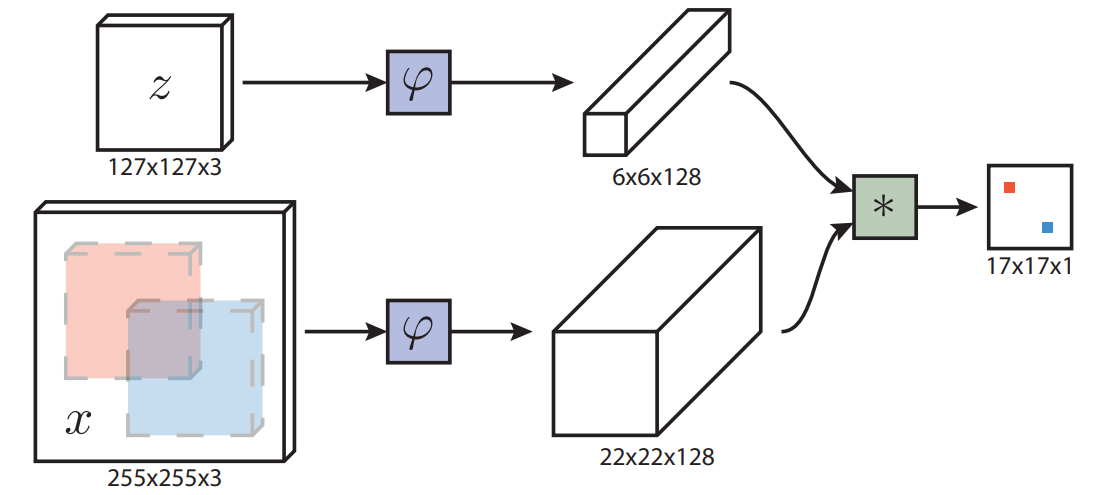
\includegraphics[width=0.75\textwidth]{Img/related/SiamFC.png}
\caption{SiamFC}
\end{figure}

\begin{figure}
\centering
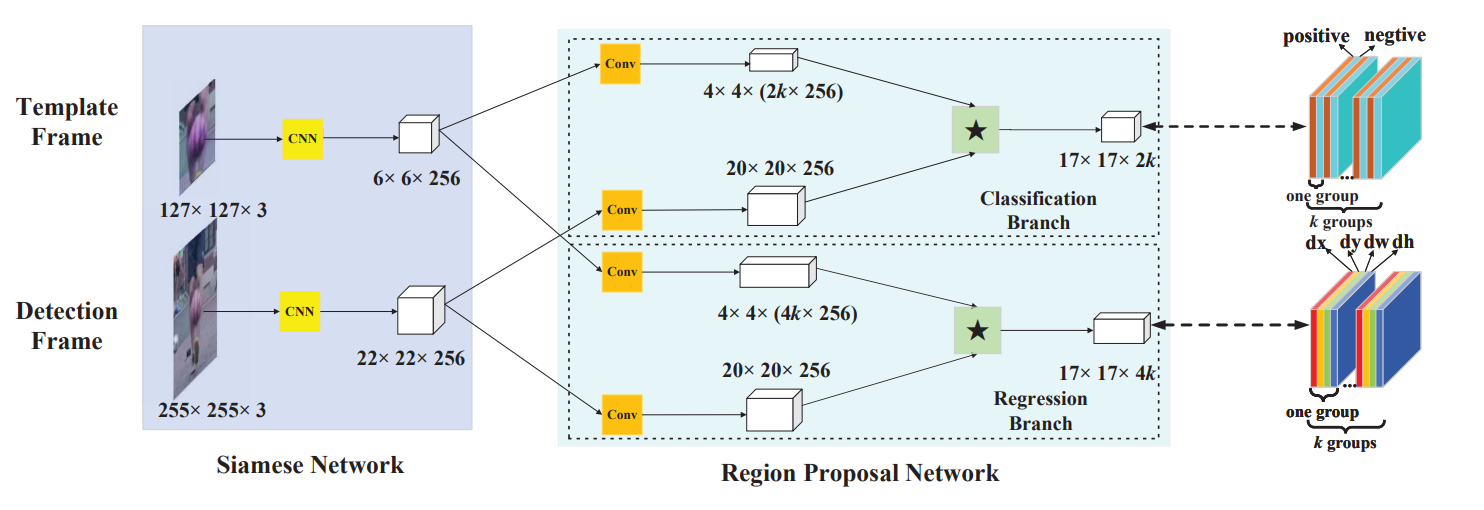
\includegraphics[width=0.75\textwidth]{Img/related/SiamRPN.png}
\caption{SiamRPN}
\end{figure}

\begin{figure}
\centering
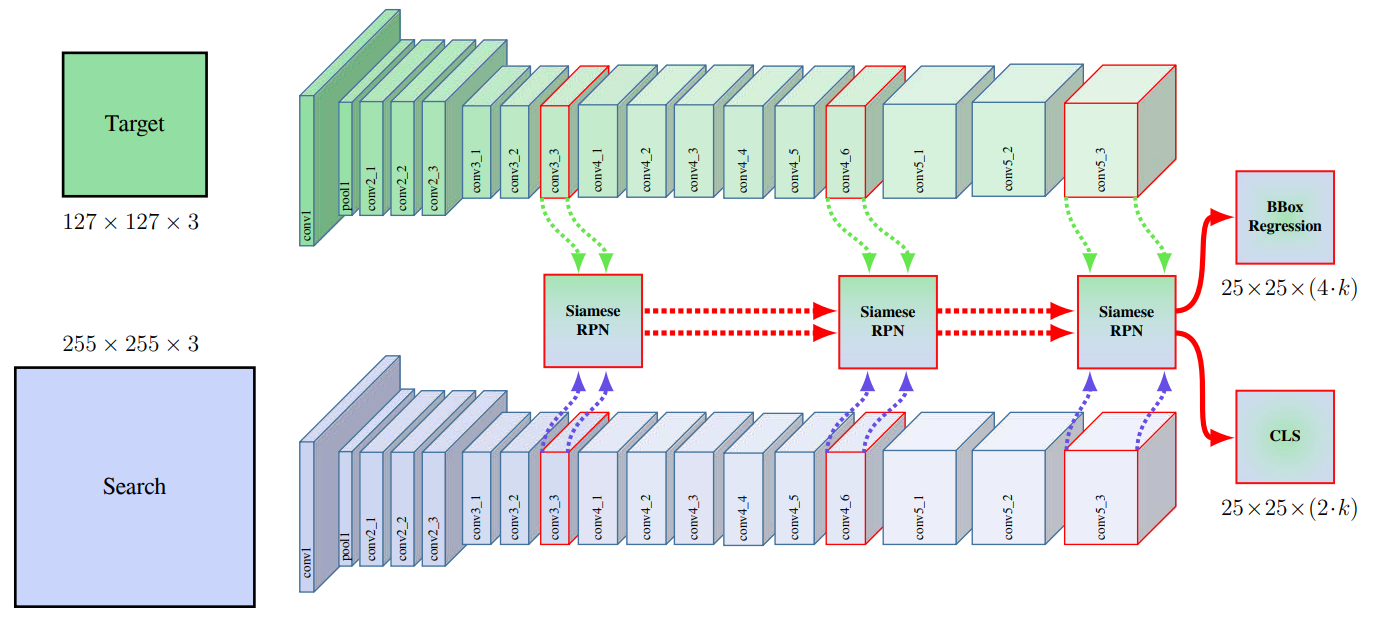
\includegraphics[width=0.75\textwidth]{Img/related/SiamRPN++.png}
\caption{SiamRPN++}
\end{figure}

\begin{figure}
\centering
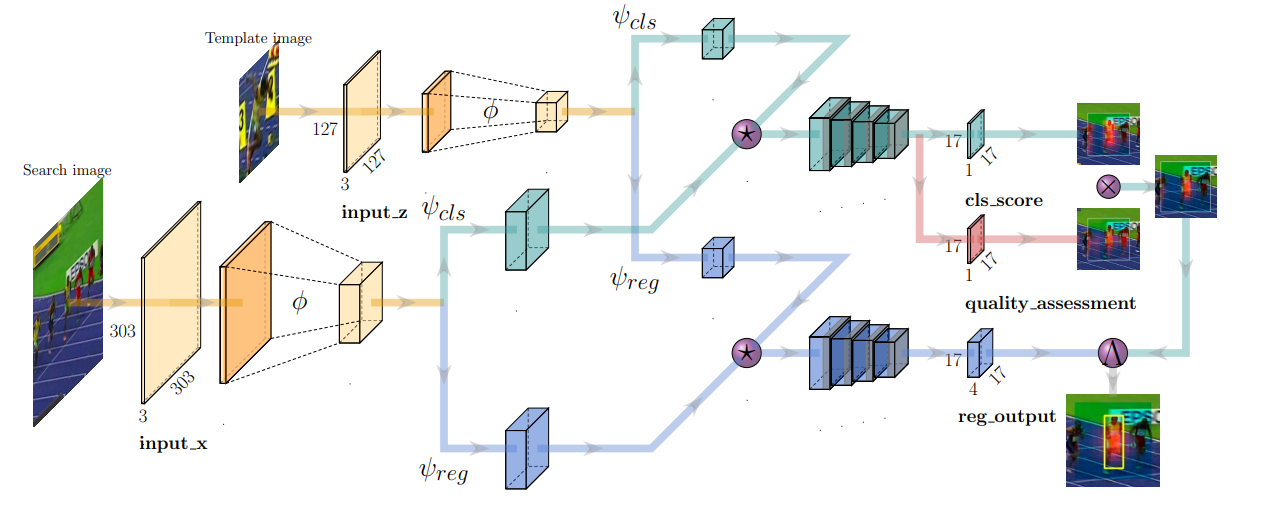
\includegraphics[width=0.75\textwidth]{Img/related/SiamFC++.png}
\caption{SiamFC++}
\end{figure}
\fi
\section{本文涉及的视觉目标跟踪数据库}
为了衡量不同视觉目标跟踪算法的效果,需要形成公平、统一的衡量标准。世界上许多研究机构都发布了不同的视觉目标跟踪数据库用于测试各种视觉目标跟踪算法的性能。目前针对视觉目标跟踪任务常用的数据集有 Object Tracking Benchmark(简称 OTB)\cite{OTB} 数据集、Visual Object Tracking(简称 VOT)\cite{VOT2015} 挑战赛数据集和大规模通用视觉目标跟踪数据集 GOT-10k \cite{GOT-10k} 等。
%引入了视觉跟踪基准数据集,以提供对单对象跟踪算法的公正和标准化的评估。
这些基准数据库可评估跟踪器在短期目标跟踪或长期目标跟踪时的表现,包含各种序列、属性和类别。常见的属性包括光照变化(IV),比例变化(SV),遮挡(OCC),形变(DEF),运动模糊(MB),快速运动(FM),平面内旋转(IPR),平面外旋转(OPR),目标出画面(OV),背景混杂(BC),低分辨率(LR),宽高比变化(ARC),相机运动(CM),完全遮挡(FOC),部分遮挡(POC) ,相似目标(SIB),视角变化(VC),表面遮挡(SC),透明度(TR),形状(SH),运动平滑度(MS),低对比度(LC),相机变焦(ZC),长时间(LD),阴影变化(SHC),闪光灯(FL),弱光(DL),相机抖动(CS),旋转(ROT),快速背景变化(FBC),运动变化(MOC),物体颜色变化(OCO),场景复杂度(SCO),绝对运动(AM),尺寸(SZ),相对速度(RS),快速摄像机运动(FCM),物体运动(OM),物体模糊(OB),长期遮挡(LOC),小物体(SOB)和长期跟踪(LT)等。通过不同的评估协议,现有的视觉跟踪基准可以评估现实场景中跟踪器的准确性和鲁棒性。统一的评估协议有助于跟踪器的直观比较和开发。下面简要介绍最流行的视觉跟踪基准数据集和评估指标。
\subsection{短期目标跟踪数据集}
作为最早的目标跟踪基准之一,OTB2013 \cite{OTB} 使用 50 个完全注释的序列构建跟踪数据集,定义了 11 中视觉属性并对视频序列进行了分类标注。这些属性包括光照变化、低分辨率、尺度变化、背景干扰、目标遮挡、目标出画面、非刚性形变、平面内旋转、平面外旋转、运动模糊以及快速运动。OTB2015 \cite{OTB2015} 在 OTB2013 数据集上进行了扩展,旨在实现无偏的性能比较。
%在 OTB 中,使用精确度和成功率对跟踪器进行定量评估。
为了定量评价跟踪算法性能,OTB 数据集提出距离精度曲线(Precision Plot)以及重叠率成功曲线(Success Plot)。
在早期衡量跟踪算法精确度的评价指标中,一种广泛使用的方法是中心位置误差,通过计算跟踪器预测的中心点位置与对应帧的真实目标位置中心之间的平均欧式距离来估计算法性能。但当跟踪器丢失对目标的跟踪时,通常输出位置可能是随机分布的,因此上述平均误差值可能无法正确衡量跟踪性能。跟踪器预测的目标中心位置与真实目标中心位置在给定阈值距离内的帧数百分比是测量跟踪性能的更好度量,OTB 数据集使用在阈值为 20 像素时的平均距离精度作为度量指标。在 OTB 中采用另一个评估指标是平均重叠率,通过计算不同重叠率阈值下的图像帧数比例来绘制重叠率成功曲线。通过在该曲线下将不同阈值的成功率采样取平均可以计算成功图的曲线下面积,该指标是 OTB 数据集进行排名的主要依据。
为了比较视觉跟踪器在彩色帧序列上的性能,Temple-Color 128(简称为 TColor128 或 TC128)\cite{TC128} 收集了 128 个完全注释的视频序列,其中有 78 个视频与 OTB 数据集不同。
ALOV 数据集 \cite{ALOV} 包括 304 个短视频和 10 个长视频,强调具有挑战性的视觉跟踪场景,涵盖各种视频序列和属性。这些视频片段是从 YouTube 视频中选择的。
%ALOV 的视频已根据其属性之一进行了分类,尽管在 OTB 数据集中,每个视频都具有几种视觉属性。
VOT 数据集 \cite{VOT2015} 提供了一个与现有数据集不同且足够小的数据集,并通过旋转边框和视觉属性对每帧进行了注释。为了快速而直接地评估不同的视觉跟踪方法,VOT 采用视觉跟踪交换(TraX)协议 \cite{TraX},该协议不仅可以准备数据,运行实验并执行分析,还可以检测跟踪失败(即跟丢目标),并且在每次失败后重新初始化跟踪器,以评估跟踪的鲁棒性。
为了更好地了解跟踪器的性能,VOT 为视频序列中的每个帧手动或半手动标记了五个视觉属性,这些属性反映了表观退化的特定挑战:(1)遮挡,(2)照明变化,(3)运动变化,(4)尺寸变化,(5)摄像机运动。如果某帧不属于于五个退化中的任何一个,则将其表示为(6)未退化。
VOT 采用两个正交的评价指标:精确度和鲁棒性。精确度衡量跟踪器预测的边界框与真值边界框的重叠程度,而鲁棒性衡量的是跟踪器在跟踪过程中丢失目标的次数。
TrackingNet \cite{muller2018trackingnet} 是一个大规模基准数据集,包括 500 个视频,超过 1400 万个垂直边框注释。视频采样于 YouTube 的真实场景,具有丰富的目标类别分布。
为了跟踪行人和刚性物体,NUS-PRO 数据集 \cite{NUS} 提供了来自 YouTube 的 365 个视频序列,这些视频序列主要由移动摄像机捕获,并注释了每帧中目标被遮挡的程度,包括无遮挡、部分遮挡和完全遮挡。
NfS 数据集 \cite{Nfs} 提供了来自真实场景的视频序列,具有更高的帧率(240 FPS)。这些视频可以通过手持式 iPhone/iPad 摄像机录制,也可以通过 YouTube 视频录制。
GOT-10k \cite{GOT-10k} 包括超过一万个视频片段,分为 563 类运动目标和 87 类运动模式,以尽可能覆盖现实情况中的各种挑战性模式,并带有超过 150 万个手动标记的边界框,从而可以对深度跟踪器进行统一训练和稳定评估。
在 GOT-10k 采用的跟踪器评估协议中,训练集和测试集的物体类别是零重叠的。该协议避免了评估结果的偏差,并促进了跟踪器开发的规范化。
GOT-10k 构建了一个大型的稳定测试集,具有 84 类运动目标和 31 类运动模式。GOT-10k 选择广泛使用的平均重叠(AO)和成功率(SR)作为指标。平均重叠表示所有真实边框和预测边框之间重叠的平均值,而成功率表示重叠超过阈值(如0.5)的成功跟踪的帧的百分比。
%最后,TracKlinic \cite{TracKlinic} 引入了一个工具包(从 OTB2015,TC128 和 LaSOT 收集),该工具包每个序列仅包含一个具有挑战性的因素来评估视觉跟踪器。它还提供了两个具有挑战性的 O-B 和 O-R 属性,包括背景杂波和旋转的遮挡。
UAV123 \cite{mueller2016benchmark} 提供了一个低空航拍跟踪数据集,包含真实的和合成的高清视频序列。这些视频由安装在专业级飞行机器人、小型低成本飞行机器人或模拟器上的摄像机捕获。
DTB \cite{DTB} 是由飞行机器人或无人机捕获的数据集,视频为 RGB 格式。由于摄像机经常发生突然移动,视频中目标位置往往会发生很大的位移。
%BUAA-PRO 数据集 \cite{BUAA-PRO} 是基于分割的基准数据集,用于解决边框中不可避免的非目标信息的问题。该数据集利用了基于级别的遮挡属性的基于分段掩码的版本。
UAVDT 数据集 \cite{UAVDT} 提供了具有不同场景(例如不同的天气条件、摄像机视角、飞行高度)的航拍数据集,重点关注行人和车辆。
此外,VisDrone 数据集 \cite{VisDrone} 包括现实世界中不同无人机平台捕获的视频。对于小目标跟踪,Small-90 数据集 \cite{Small} 收集了来自其他视频跟踪数据集中的航拍视频。在 Small-90 数据集的基础上,通过添加 22 个更具挑战性的序列,构成了数据集 Small-112 数据集 \cite{Small}。 
\subsection{长期目标跟踪数据集}
OxUvA 数据集 \cite{OxUvA} 从 YouTubeBoundingBoxes(简称 YTBB)\cite{YTBB} 中采集了时长 14 小时的视频。由于长期跟踪过程中目标会频繁消失,该数据集提供标签以表明某些帧中不存在目标。
TLP 数据集 \cite{TLP} 从 YouTube 中收集了持续时间更长的高分辨率视频,为研究跟踪一致性提供了可能。然而,目标消失在 TLP 数据集中并不常见。
因此,LTB-35 \cite{LTB} 提出了一个丰富的长期跟踪数据集,具有频繁的目标消失(每个视频平均十二次消失)现象。
大规模单目标跟踪数据集 LaSOT \cite{LaSOT} 致力于解决现有数据集中存在的规模小、视频质量差、类别偏差等问题。该数据集中的每个类别具有相同数量的视频。训练和测试子集分别包括 1120 段(2.3M 帧)和 280 段(690K 帧)视频序列。
%作为 UAV-123 数据集的子集,UAV20L 是一个航拍数据集,为小目标跟踪提供了困难的场景。此外,
VisDrone-2019/2020L \cite{VisDrone} 提出了一个小目标跟踪数据集,其中包括拍摄于白天的 12 段视频和拍摄于晚上的 13 段视频。% Deep Learning for Visual Tracking: A Comprehensive Survey

\iffalse
\subsection{OTB 视觉目标跟踪数据集}
OTB 使用50个完全注释的序列构建跟踪数据集,以方便跟踪评估。
OTB 定义了 11 中视觉属性并对视频序列进行了分类标注。这些属性包括:括光照变化、低分辨率、尺度变化、背景干扰、目标遮挡、目标出画面、非刚性形变、平面内旋转、平面外旋转、运动模糊以及快速运动。

在 OTB 中,使用 presicion 和 success rate 进行定量分析。此外,从两个方面评估跟踪算法的鲁棒性。

\textbf{精度图} 在衡量跟踪算法精确度评价指标中,一种广泛使用的方法是中心位置误差,其定义是:预测的目标中心位置与人工标记的真实目标中心位置的平均欧几里得距离。然后,使用一个视频序列的所有帧的平均中心位置误差来代表该视频的总体性能。但是,当跟踪器丢失目标时,预测的位置可能是随机的,因此上述平均误差值可能无法正确衡量跟踪性能。最近,采用精度图来衡量整体跟踪性能。它显示了估计位置在地面真相的给定阈值距离内的帧的百分比。作为每个跟踪器的代表精度得分,我们使用阈值=20像素的得分。
\textbf{成功图} 另一个评估指标是边界框重叠。给定预测的边界框和真实边界框,重叠分数定义为这两个边框的交并比。为了衡量跟踪器在由多帧组成的视频上的性能,我们计算边框重叠大于给定阈值的帧的数量。成功图反映了成功的帧数在给定阈值(0到1之间)的比率。使用特定阈值(例如to = 0.5)的一个成功率值进行跟踪器评估可能不公平或不典型。 相反,我们使用每个成功图的曲线下面积(AUC)对跟踪算法进行排名。

\subsection{VOT 视频跟踪数据集}
VOT 挑战的目标是用户在序列的第一个图像中手动初始化跟踪器的情况。万一跟踪器发生故障(例如,偏离目标),则用户将在故障图像处重新初始化跟踪器。因此,需要跟踪器为序列的每个帧预测目标的单个边界框。通过将预测的边界框与地面真值注释进行比较,可以自动检测到故障,如果重叠为零,则宣布为故障。
为了更好地了解跟踪器的性能,我们为每个选定序列中的每个帧手动或半手动标记了五个视觉属性,这些属性反映了外观退化的特定挑战:(1)遮挡,(2)照明变化,(3)运动变化,(4)尺寸变化,(5)摄像机运动。如果特定帧不对应于五个降级中的任何一个,则将其表示为(6)未降级。
基于最近对广泛使用的性能指标的分析[44],我们选择了两个正交指标:(1)准确性和(2)鲁棒性。精度测量跟踪器预测的边界框与地面真值边界框的重叠程度。另一方面,鲁棒性衡量的是跟踪器在跟踪过程中失去目标的次数。

\subsection{GOT-10k 视频跟踪数据集}
GOT-10k建立在WordNet结构的骨干基础上[1],它填充了563多个运动对象和87个运动模式,旨在为开发与类无关的通用短期跟踪器提供统一的
和评估平台。
GOT-10k提供了10,000多个视频片段,并带有超过150万个手动标记的边界框,从而可以对深度跟踪器进行统一训练和稳定评估。
GOT-10k首次引入了用于跟踪器评估的单发协议,其中训练和测试课程是零重叠的。该协议避免了对熟悉对象的偏倚评估结果,并促进了跟踪器开发的一般化。
我们构建了一个大型的稳定测试集,其中包括420个视频,这些视频属于84个对象类和31个运动类。我们选择广泛使用的平均重叠(AO)和成功率(SR)作为指标。 AO表示所有地面和估计边界框之间的重叠的平均值,而SR表示重叠超过阈值(例如0.5)的成功跟踪帧的百分比。
\fi
\section{本章小结}
本章对基于深度学习的主流视觉目标跟踪方法进行了详细介绍。本章将基于深度学习的跟踪器划分为以下类别:基于深度特征的相关滤波跟踪器、基于生成对抗网络的跟踪器、基于图卷积网络的跟踪器、基于循环神经网络的跟踪器、基于脉冲神经网络的跟踪器、基于孪生网络的跟踪器、基于强化学习的跟踪器、基于元学习的跟踪器、基于无监督学习的跟踪器、基于注意力机制的跟踪器和基于串并联或级联结构的跟踪器,分析了这些方法的原理和各自特点。本章还介绍了常用的视觉目标跟踪数据库,用于验证本文所提方法的有效性。